\section{Revisiting OpenStack: towards a massively distributed IaaS manager}

% - OpenStack is an open-source IaaS managers project.
% - It provides all mechanisms that allow organization to host private infra.

\begin{figure*}
	\centerline{
	 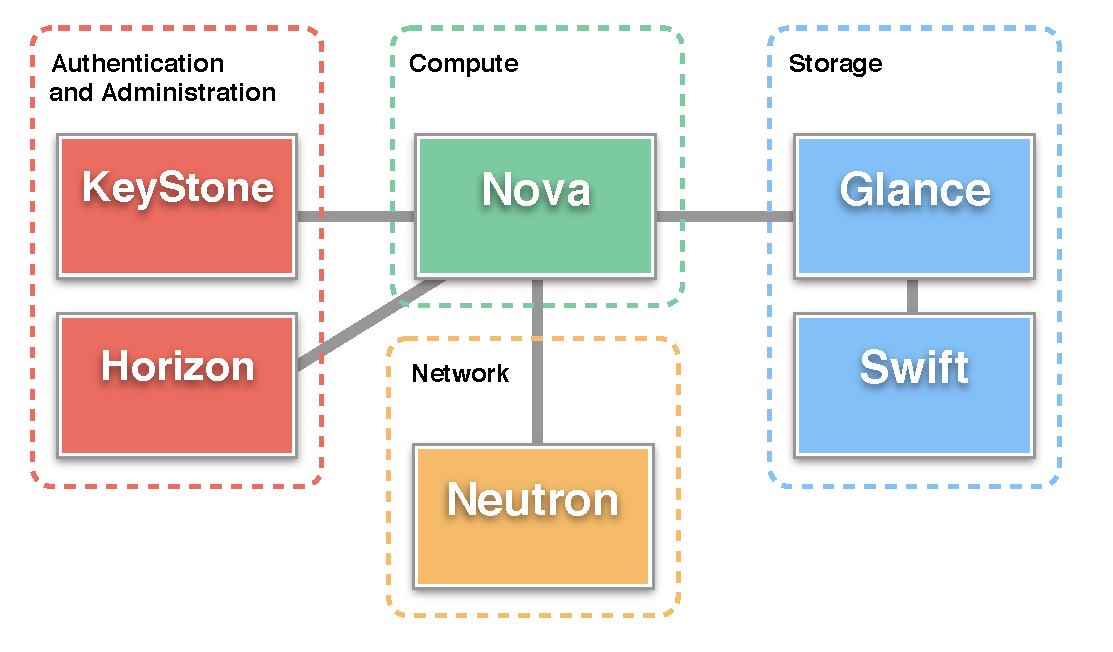
\includegraphics[width=0.75\linewidth]{Figures/openstack_architecture.pdf}
  }
	\caption{Architecture of OpenStack.}%
	\label{fig:openstack_architecture}%
	%\vspace*{-.8cm}
\end{figure*}

In Section \ref{sec:anatomy_lucos} we proposed a design for the LUC-OS 
that leverages a reference architecture, this section now considers the 
possibility of building the LUC-OS over existing mechanisms. OpenStack is an 
open-source project that aims at developing a self sufficient IaaS manager, 
containing all mechanisms that are suitable to build a private Cloud. OpenStack 
is composed of several services (nova, swift, Quantum, Glance, ...) following 
the "shared nothing architecure" principle, meaning that each service is 
independent and thus shares no state with other services. In this way, 
inter-services collaboration is performed by exchanging message through an AMQP 
(Advanced Message Queuing Protocol) based bus: each service has its own queue, 
and it collaborates with others by sending messages to their queues. This offers
the advantage of easily plugging additional components: when a default service 
becomes no more suitable with system's needs, it can be naively replaced by 
another custom service, as long as the newer service consumes messages destined 
to the older one, and in turn produces messages expected by collaborators.

% - As developing an IaaS manager is an herculean work, we want to reuse
%   existing components.
% As developing an IaaS
% manager is an herculean work, we propose to adapt OpenStack in order to base the
% LUC-OS over it. According to section \ref{sec:anatomy_lucos}, if OpenStack 
% respects the reference architecture then it means that it can be a base for the
% LUC-OS.

% - Figure representing OpenStack's architecture (Nova, Glance, Swift, Neutron, 
%   KeyStone, ...).


% - This architecture can be mapped to Moreno's architecture:
%    * Nova -> Compute manager
%    * Glance + Swift -> Storage manager
%    * Neutron -> Network manager 
%    * KeyStone, Horizon -> Authentication + Administration
% - Thus, it is possible to leverage the architecture introduced in section 3
%   over OpenStack.
Figure \ref{fig:openstack_architecture} depicts OpenStack's architecture by 
comparing its main components with the reference architecture from Section 
\ref{sec:moreno}: \emph{Nova} is very close to what is specified for the 
\emph{Compute manager} (Nova includes a static scheduler), the reunion of 
\emph{Glance} with \emph{Swift} and a DHT corresponds to the \emph{Storage 	
manager}, \emph{Neutron} exactly corresponds to the \emph{Network manager} and 
finally \emph{KeyStone} and \emph{Horizon} fits with 
\emph{Administrative tools}, \emph{Information manager} and 
\emph{Accounting/auditing}.

\subsection{Instantiating the LUC-OS over OpenStack}
\label{sub:sec:revisiting_openstack}

% - In section 3, we planned to deploy a LUC-OS agent per node of the 
%   infrastructure.
% - In this section we explain how we instantiate a first prototype of the 
%   LUC-OS over OpenStack.

In Section \ref{sec:lucos}, we exposed that the LUC-OS will rely on a 
multi-agent architecture: each compute node of the infrastructure will run an
instance of this agent. In this Section we explain how we instantiate a first
prototype of the LUC-OS over OpenStack and Figure \ref{fig:luc_os_over_os} 
exposes how the LUC-OS agent articulates with OpenStack.

\begin{figure*}
	\centerline{
	 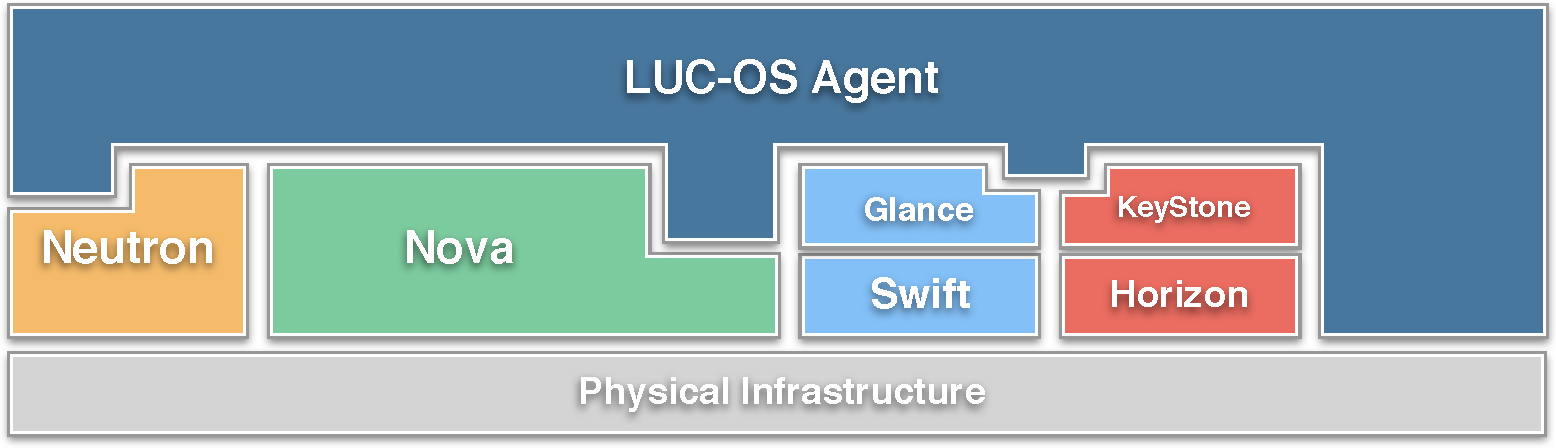
\includegraphics[width=0.95\linewidth]{Figures/lucos_over_openstack.pdf}
  }
	\caption{LUC-OS over OpenStack.}%
	\label{fig:luc_os_over_os}%
	%\vspace*{-.8cm}
\end{figure*}

% - LUC-OS: each service comes with a software interface that must be respected
%   by implementations.
% - Challenge: respect LUC-OS's interfaces and maximize the reuse of OpenStack.
%    1) LUC-OS -> OpenStack
%    2) OpenStack -> LUC-OS 
Each service composing the LUC-OS architecture defines a software interface 
that must be respected by its implementations. Hence for a given service of the
LUC-OS and its equivalent in OpenStack, the challenge is to both respect these
interfaces and maximize the reuse of tools provided by OpenStack. 

We see two ways to meet this challenge: the first one is to adapt the interface 
of the LUC-OS's service to its equivalent in OpenStack: this enables to entirely
and directly reuse implementations given by OpenStack. The second strategy is
to adapt OpenStack's implementation by changing some of its parts, in order to 
respect the interface given by the LUC-OS. These two integration strategies are
applied on a case-by-case basis according to the difficulty of adapting the 
OpenStack tool. 

The first integration strategy can be illustrated with \emph{Swift}: this 
component provides fault-tolerance mechanisms, already works in a peer to peer
manner and thus meets our requirements for the \emph{Distributed Data Store}. As
we plan to make the \emph{Storage service} directly use it, the first 
integration strategy is the best suited for this example.

Inversely, \emph{Nova} is typically deployed on centralized service nodes and 
has been designed in a way which does not fit with the peer to peer (p2p) 
paradigm: reusing features given by \emph{Nova} in the LUC-OS will require to 
replace some of its parts (nova-scheduler will be replaced by a p2p scheduler 
like DVMS \cite{quesnel:ispa2013}), which corresponds to the second strategy. 
The same will happen with \emph{Neutron}, \emph{Glance}, \emph{KeyStone} and
\emph{Horizon}: all the parts of these services that does not fit with a peer to
peer functioning will be replaced by more suitable mechanisms.

\subsection{Detailled use case of a first LUC-OS prototype}
\label{sub:sec:revisiting_openstack}


% - Connection to a node -> VE request.
% - One VM spawner get the request, selects severs that will host the VE.
% - A virtual LAN is create: each server of the VE shares the networking effort.
%   This will be done with Neutron or Mininet / Vine.
% - When the VLAN is created -> VMs creation stage begins:
%    - VMs' images are uploaded on each node of the VE.
%    - VMs' images are are added in swift and Glance.
%    - VM creation, interconnected with others through the VE's vlan.
%    - VM are started.
% - When one of the compute nodes [is overloaded], the scheduler will resolve 
%   the overload
% - The Scheduler selects underloaded servers and migrate some VMs on these 
%   underloaded servers.
% - Challenge: these new servers will have to share the effort of hosting VEs:
%   a vlan agent is started on theses servers.
When a user wants to create a VE that contains several VMs, it has to connect to
one of the compute nodes of the LUC-OS infrastructure and create a VE request
containing a description of VMs to create. One instance of the \emph{VM spawner}
processes this request: a set of servers is elected to share the effort of 
hosting the VE. A new virtual network is created to interconnect VMs of the VE:
each agent will share the interconnecting effort by hosting a virtual network 
agent. This agent will be leveraging \emph{Neutron} or \emph{Mininet/Vine}.

When the virtual lan is created the VMs creation stage starts: VMs images that 
have been specified in the VE request are uploaded on the compute nodes of the 
VE and added in their respective \emph{Glance}. Subsequently, VMs are created 
configured and and interconnected through the previously created VLAN. Once all
the preceding tasks have been performed, VMs are started.

\begin{figure*}
	\centerline{
	 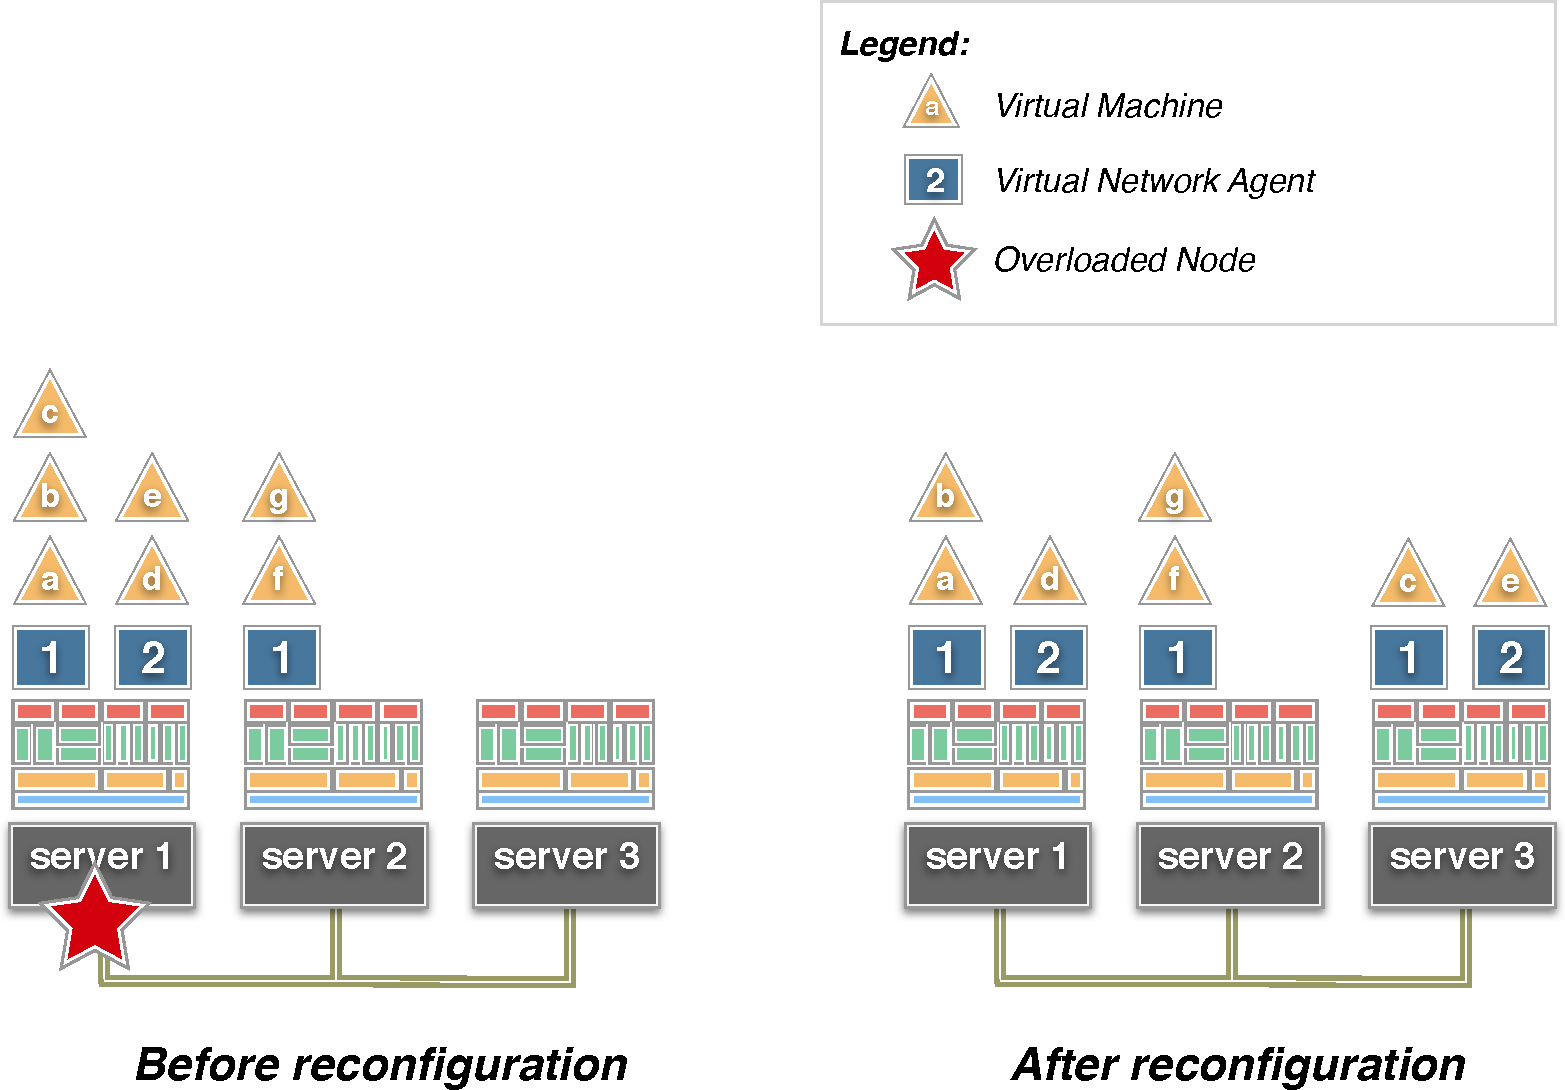
\includegraphics[width=1.0\linewidth]{Figures/lucos_reconfiguration.pdf}
  }
	\caption{Reconfiguration process that occurs when a compute node is 
	overloaded.}%
	\label{fig:lucos_reconfiguration}%
	%\vspace*{-.8cm}
\end{figure*}

\newpage

This configuration doesn't change until the VMs hosted on a compute node are
consuming more resource than can be produced: the compute node becomes 
overloaded. Figure \ref{fig:lucos_reconfiguration} illustrates this situation: 
\emph{Server 1} becomes overloaded while \emph{Server 2} and \emph{Server 3} are
underloaded. \emph{Server 1} requests the \emph{Scheduler} to balance the VM 
hosting effort with other nodes of the infrastructure. To do so, the 
\emph{Scheduler} starts the search of some underloaded servers, finds 
\emph{Server 2} and \emph{Server 3} and, by means of VM migrations, produces a 
new \emph{VMs/Compute nodes} mapping that satisfy ressources requested VMs of
\emph{Server 1}: VM \emph{c} and \emph{e} are migrated on \emph{Server 3}. This
instance also points another challenge that must be resolved: a server selected 
by the \emph{Scheduler} may not be already part of the VE. Indeed, before the 
reconfiguration \emph{Server 1} and \emph{server 2} were parts of VE \emph{1},
VE \emph{2} was only hosted by \emph{server 2} and \emph{Server 3} was not 
taking part at any VE hosting effort. After the reconfiguration, \emph{Server 3} 
is now taking part at the hosting effort of VE \emph{1} and \emph{2} and two 
\emph{Virtual Network Agents} are started on it.

\subsection{How a service like Nova can be revisited to become part of the 
LUC-OS?}
\label{sub:sec:nova_lucos}

Nova is the component that manages compute nodes in a centralized manner by
processing messages received through an AMQP bus. As it has been designed to 
work in a centralized manner, we want to revisit it in a way that enables its
integration in the LUC-OS: mechanisms that needs to be distributed will be 
delagated to the LUCOS.

A good instance is the scheduling of VMs: with "vanilla Openstack", Nova decides
on which host VMS will runs (static scheduling). As this functionning doesn't
fit with the requirements of the LUC-OS (i.e scalability and fault tolerance),
\emph{nova-scheduler} will be replaced by a custom python class that will 
implements a scheduler that delegates the all static scheduling decision to the
\emph{VM Spawner}: messages that are sent by others OpenStack's service (
typically \emph{Horizon} transforms user's interactions into messages that are
sent to \emph{Nova} through the AMQP bus) sent to \emph{nova-scheduler} will be
accepted by this custom scheduler, delegated to the LUC-OS and in return 
responses from the LUC-OS will be in turn transmitted to other OpenStack 
components.

As this custom scheduler block, that extends the interface given by Openstack, 
is tightly coupled with the LUC-OS, it can then be considered as part of the
LUC-OS. The same method will be applied to all other services composing the 
LUC-OS.







